%%%%%%%%%%%%%%%%%%%%%%%%%%%%%%%%%%%%%%%%%%%%%%%%%%%%%%%%%%%%
% Name: XeTeX+xeCJK日常使用模板
% Author: Lox Freeman
% Email: xiaohanyu1988@gmail.com
%
% 本文档可以自由转载、修改,希望能给广大TeXer的中文之路提供一些方便。
%%%%%%%%%%%%%%%%%%%%%%%%%%%%%%%%%%%%%%%%%%%%%%%%%%%%%%%%%%%%

\documentclass[a4paper, 12pt, openany]{book}

\usepackage{times}
\usepackage{upquote} % 解决lstlisting中单双引号显示

	% To add Chinese character encoding
\usepackage{xunicode, xltxtra}
\setmainfont[Mapping=tex-text]{AR PL KaitiM GB}
\setsansfont[Mapping=tex-text]{AR PL KaitiM GB}
\XeTeXlinebreaklocale "zh"

\makeatletter
\makeatother
\setlength{\parindent}{2em}%中文缩进两个汉字位
%中文断行
\XeTeXlinebreakskip = 0pt plus 1pt

%%%%%%%%%%%%%日常所用宏包、通通放在一起%%%%%%%%%%%%%%%%%%%%%%%%%%%%
% 什么常用的宏包都可以放这里。下面是我常用的宏包,每个都给出了简要注释
\usepackage[top=2.5cm, bottom=2cm, left=2cm, right=2cm]{geometry} % 控制页边距
\usepackage{enumerate}               % 控制项目列表
\usepackage{multicol}                % 多栏显示

\usepackage[%
    pdfstartview=FitH,%
    bookmarks=true,%
    bookmarksnumbered=true,%
    bookmarksopen=true,%
    colorlinks=true,%
    citecolor=blue,%
    linkcolor=blue,%
    anchorcolor=green,%
    urlcolor=blue%
]{hyperref}

\usepackage{titlesec}                % 控制标题
\usepackage{titletoc}                % 控制目录
\usepackage{type1cm}                 % 控制字体大小
\usepackage{indentfirst}             % 首行缩进,用\noindent取消某段缩进
\usepackage{cite}                    % 支持引用
\usepackage{color,xcolor}            % 支持彩色文本、底色、文本框等
\usepackage{latexsym}                % LaTeX一些特殊符号宏包
\usepackage{amsmath}                 % AMS LaTeX宏包
\usepackage{bm}                      % 数学公式中的黑斜体
\usepackage{relsize}                 % 调整公式字体大小:\mathsmaller, \mathlarger
%\makeindex                          % 生成索引

%%%%%%%%%%%%%%%%%%%%%%%%%基本插图方法%%%%%%%%%%%%%%%%%%%%%%%%%%%
\usepackage{graphicx}                % 图形宏包
% \begin{figure}[htbp]               % 控制插图位置
%   \setlength{\abovecaptionskip}{0pt}    
%   \setlength{\belowcaptionskip}{10pt}
                                     % 控制图形和上下文的距离
%   \centering                       % 使图形居中显示
%   \includegraphics[width=0.8\textwidth]{CTeXLive2008.jpg}
                                     % 控制图形显示宽度为0.8\textwidth
%   \caption{CTeXLive2008安装过程} \label{fig:CTeXLive2008}
                                     % 图形题目和交叉引用标签
% \end{figure}
%%%%%%%%%%%%%%%%%%%%%%%%%插图方法结束%%%%%%%%%%%%%%%%%%%%%%%%%%%


%%%%%%%%%%%%%%%%%%%%%%%%%fancyhdr设置页眉页脚%%%%%%%%%%%%%%%%%%%%
\usepackage{fancyhdr}                % 页眉页脚
\pagestyle{fancy}                    % 页眉页脚风格
\setlength{\headheight}{15pt}        % 有时会出现\headheight too small的warning
%\fancyhf{}                          % 清空当前页眉页脚的默认设置
\fancyhead{}
\fancyfoot{}
\chead{学习程序设计}
%\rfoot{\thepage\ of \pageref{LastPage}}
%%%%%%%%%%%%%%%%%%%%%%%%%fancyhdr设置结束%%%%%%%%%%%%%%%%%%%%%%%


%%%%%%%%%%%%%%%%%%%%%%%%%listings宏包粘贴源码%%%%%%%%%%%%%%%%%%%%
\usepackage{listings}                % 方便粘贴源代码,部分代码高亮功能
\lstloadlanguages{}                  % 所要粘贴代码的编程语言

%%%%设置listings宏包的一些全局样式%%%%
%%%%参见http://hi.baidu.com/shawpinlee/blog/item/9ec431cbae28e41cbe09e6e4.html%%%%
\lstset{
%numbers=left,                        % 在左边显示行号
%numberstyle=\tiny,
keywordstyle=\color{blue!70}, commentstyle=\color{red!50!green!50!blue!50},
                                     % 关键字高亮
showstringspaces=false,              % 解决代码中的空格
frame=shadowbox,                     % 给代码加框
rulesepcolor=\color{red!20!green!20!blue!20},
escapechar=`,                        % 中文逃逸字符
xleftmargin=2em,xrightmargin=2em, aboveskip=1em,
breaklines,                          % 这条命令可以让LaTeX自动将长的代码行换行排版
extendedchars=false                  % 这一条命令可以解决代码跨页时,章节标题,页眉等汉字不显示的问题
}
%%%%%%%%%%%%%%%%%%%%%%%%%listings宏包设置结束%%%%%%%%%%%%%%%%%%%%


%%%%%%%%%%%%%%%%%%%%%%%%%一些关于中文文档的重定义%%%%%%%%%%%%%%%%%

%%%%数学公式定理的重定义%%%%
\newtheorem{example}{例}                                   % 整体编号
\newtheorem{algorithm}{算法}
\newtheorem{theorem}{定理}[section]                         % 按 section 编号
\newtheorem{definition}{定义}
\newtheorem{axiom}{公理}
\newtheorem{property}{性质}
\newtheorem{proposition}{命题}
\newtheorem{lemma}{引理}
\newtheorem{corollary}{推论}
\newtheorem{remark}{注解}
\newtheorem{condition}{条件}
\newtheorem{conclusion}{结论}
\newtheorem{assumption}{假设}

%%%%章节等名称重定义%%%%
\renewcommand{\contentsname}{目录}     
\renewcommand{\indexname}{索引}
\renewcommand{\listfigurename}{插图目录}
\renewcommand{\listtablename}{表格目录}
\renewcommand{\figurename}{图}
\renewcommand{\tablename}{表}
\renewcommand{\appendixname}{附录}

%%%%设置chapter、section与subsection的格式%%%%
\titleformat{\chapter}{\centering\huge}{第\thechapter{}章}{1em}{\textbf}
\titleformat{\section}{\centering\LARGE}{\thesection}{1em}{\textbf}
\titleformat{\subsection}{\Large}{\thesubsection}{1em}{\textbf}
%%%%%%%%%%%%%%%%%%%%%%%%%中文重定义结束%%%%%%%%%%%%%%%%%%%%


%%%%%%%%%%%%%%%%%%%%%%%%%一些个性设置%%%%%%%%%%%%%%%%%%%%%%
% \renewcommand{\baselinestretch}{1.3}     % 效果同\linespread{1.3}
% \pagenumbering{arabic}                   % 设定页码方式,包括arabic、roman等方式
% \sloppy                                  % 有时LaTeX无从断行,产生overfull的错误,
                                           % 这条命令降低LaTeX断行标准
\setlength{\parskip}{0.5\baselineskip}     % 设定段间距
\linespread{1.2}                           % 设定行距
\newcommand{\pozhehao}{\kern0.3ex\rule[0.8ex]{2em}{0.1ex}\kern0.3ex}
                                           % 中文破折号,据说来自清华模板

%%%%%%%%%%%%%%%%%%%%%%%%%个性设置结束%%%%%%%%%%%%%%%%%%%%%%

\usepackage[toc]{multitoc}
%%%%%%%%%%%%%%%%%%%%%%%%%正文部分%%%%%%%%%%%%%%%%%%%%%%%%%
\begin{document}
\setlength{\parindent}{2em}                    
% 设定首行缩进为2em。注意此设置一定要在document环境之中。
% 这可能与\setlength作用范围相关

%\title{学习程序设计}
%\author{Chris Pine 著}
%\date{2011年6月23日}
%\maketitle

\begin{titlepage}
\vspace*{4ex}
  \begin{flushright}
    \Huge\textbf{学习程序设计}
  \end{flushright}
  \rule{\textwidth}{.2ex}
  %\begin{flushleft}
   %Version 0.1 draft\\
   %\today
  %\end{flushleft}
  %\vspace{8ex}
  \hspace{2em}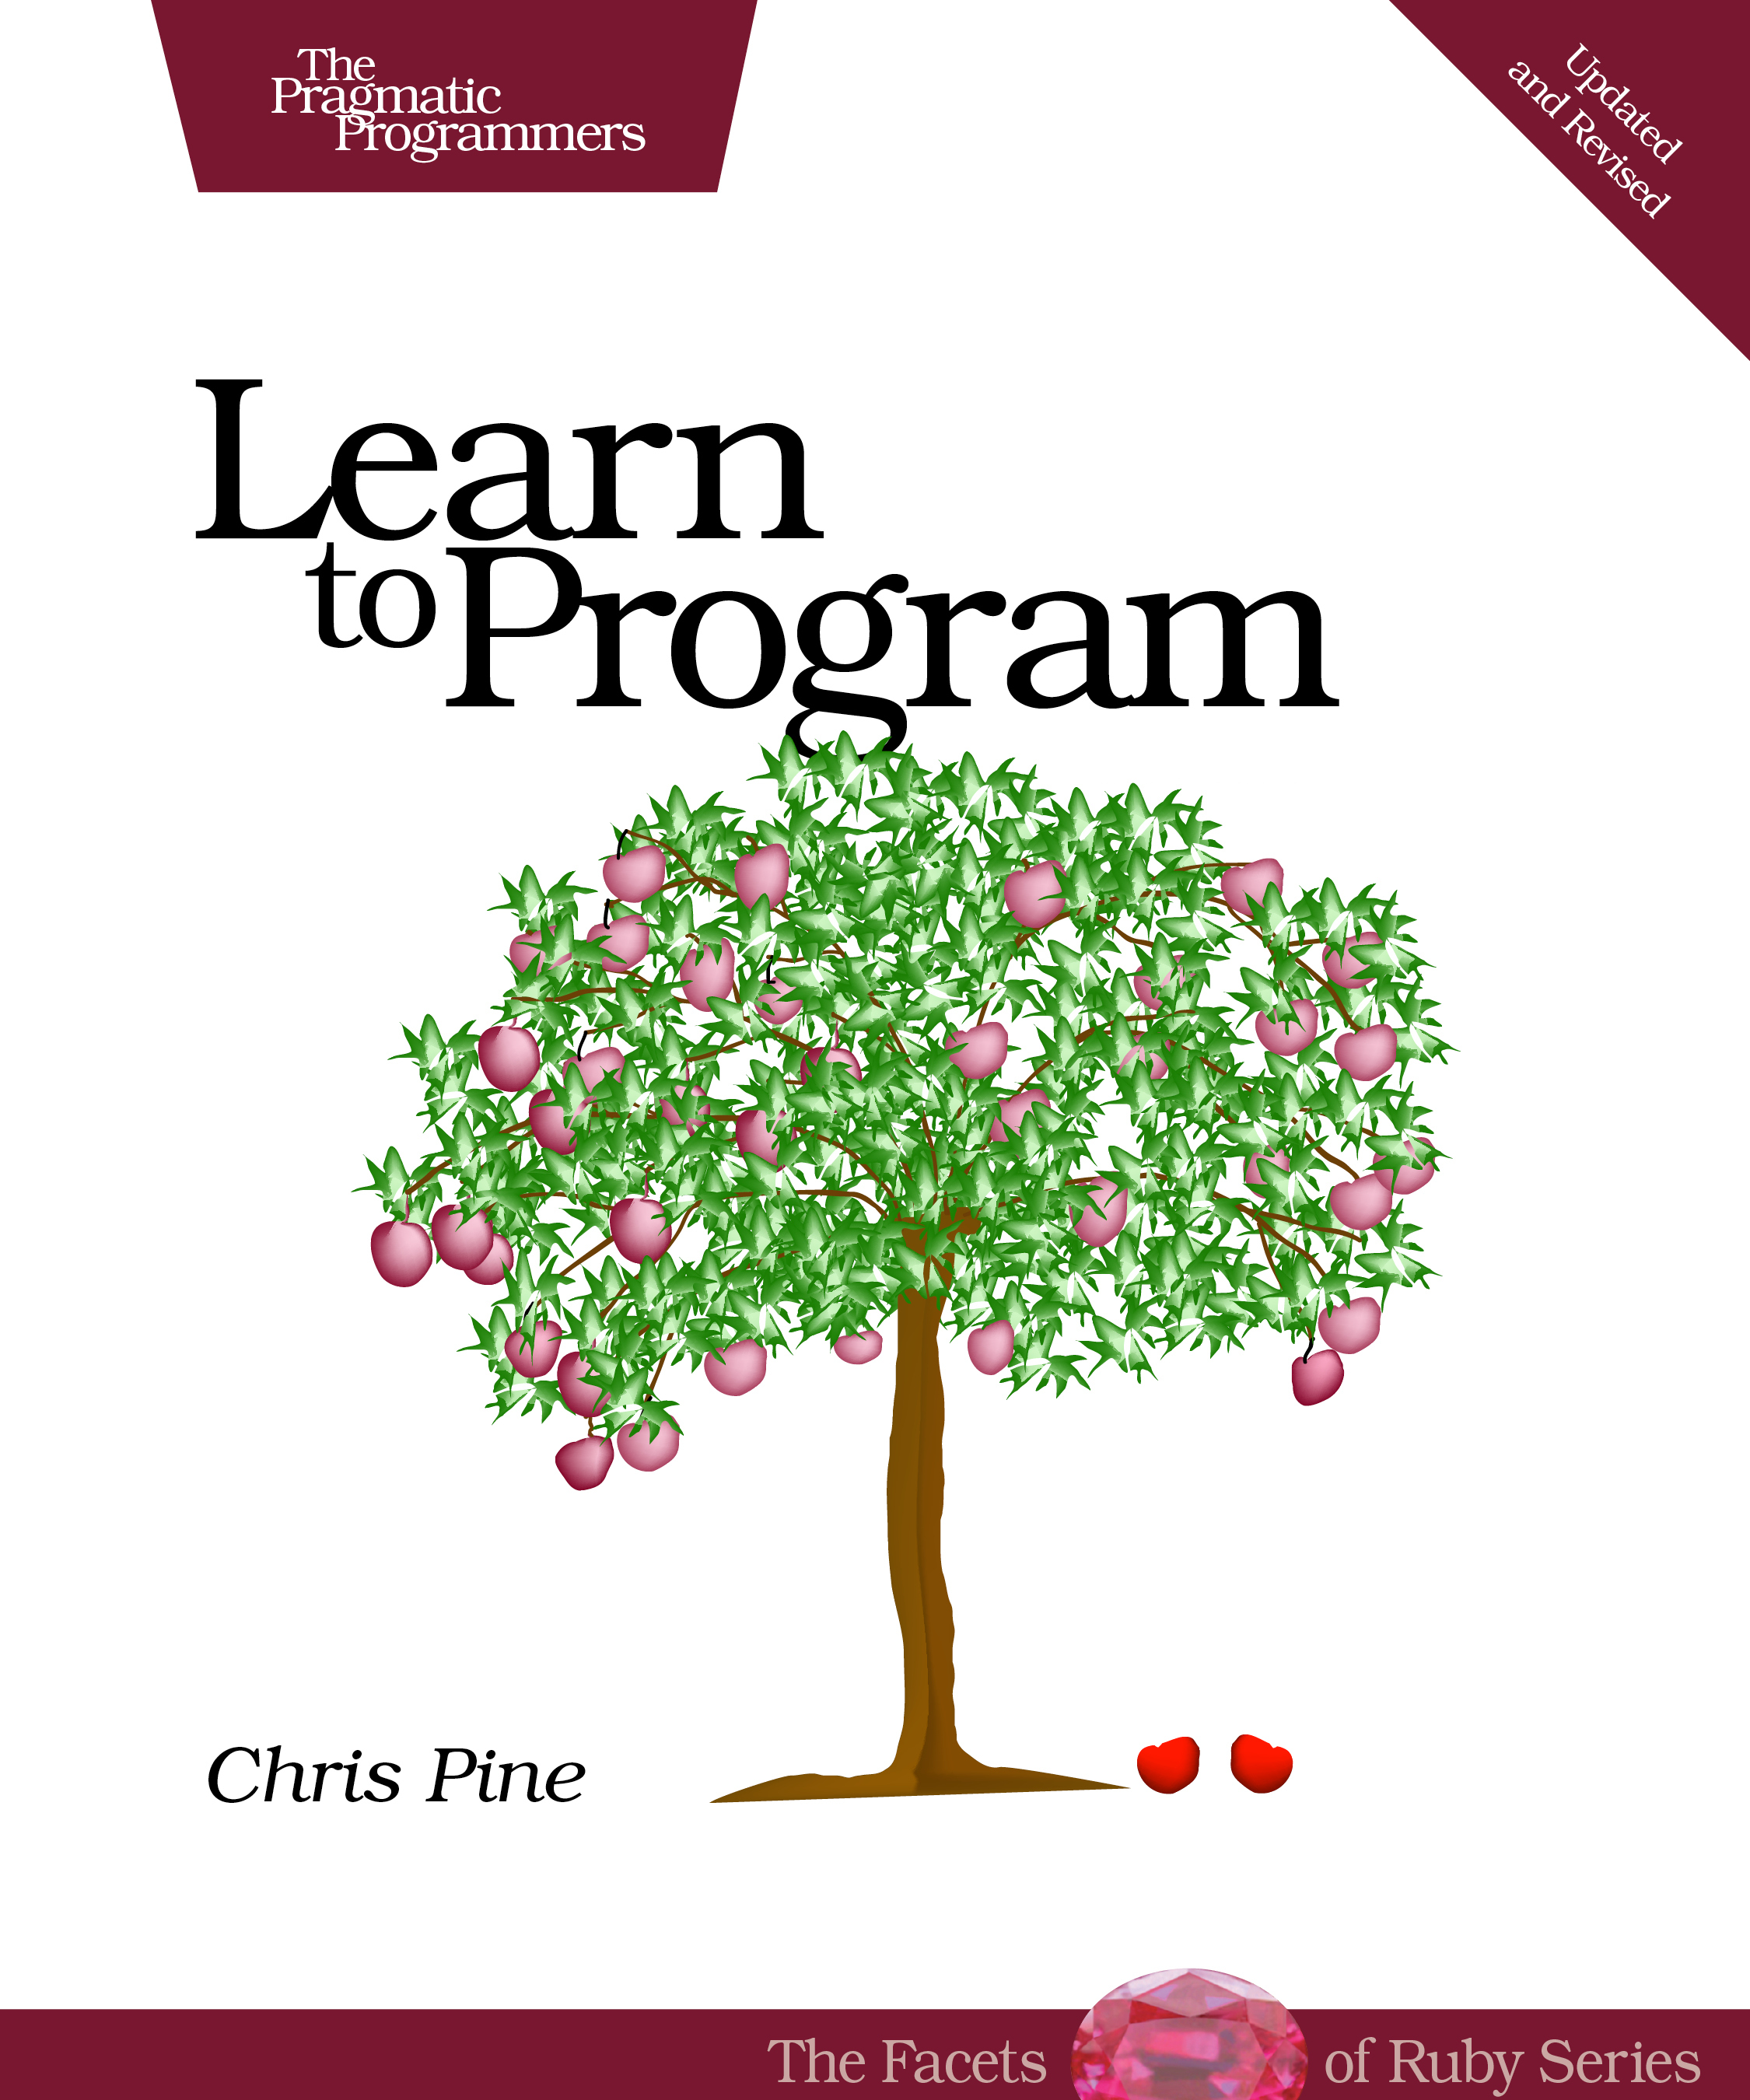
\includegraphics[scale=0.9]{cover}
  %\vspace{8ex}
  %\begin{flushright}
   % By Chris Pine 克里斯.派\\
   % Email: \texttt{chris@pine.org}
  %\end{flushright}
\end{titlepage}
\newpage

% preface
\chapter*{序}
\addcontentsline{toc}{chapter}{序}
\begin{quotation}
学而实习之,不亦乐乎!
\begin{flushright}
\textit{ -- 《论语》}
\end{flushright}
\end{quotation}
%\setlength{\parindent}{2.5em}

\begin{center}
\larger{Learn to Program 中文译本}
\end{center}

\noindent
尊敬的Pine先生:

   非常荣幸给您写了这封邮件!我是一名linux程序员,名默之。当今天阅读您的大作《学习程序设计》一书时,便萌生了一个想法\pozhehao 即将之译成中文。这样做是我的兴趣使之然,亦可给中国初学者分享ruby程序设计知识。您介意我这么做吗?
    
    献上我良好的祝愿送给您和您家人!

\begin{flushleft}
致敬!\\
\end{flushleft}

\begin{flushright}
默之 于珠海\\
2010年5月22日
\end{flushright}


\tableofcontents
\newpage

% chapter 0
\chapter{初步}

当使用计算机编程时,您必须“说”计算机能理解的语言,也就是程序设计语言。然而世界上有众多不同的程序语言,其中许多语言非常出色。在本指南中,我挑选了自己最喜爱的程序设计语言\pozhehao{Ruby}。

除了是我最喜欢的程序设计语言,Ruby也是我见过(我见识过许多程序设计语言)最简易的程序设计语言。事实上,这也是我写这本指南的真实原因。之前我没打算写一本指南,然后选择了Ruby语言因为它是我的最爱。相反,我发现Ruby的简易性而决定应该为初学者写一份指南。这正是Ruby的简易性促使这本指南的诞生,而不是我的爱好。(使用其它程序设计语言编写一本简易的指南,比如C++或Java,将会花费大量的纸张。)但是不要因为Ruby的简易性而认为它是一种初学者编程语言。Ruby是一种十分强大且满足专业需求的程序设计语言。

当你使用人类语言书写东西时,你所书写的称之为文字。而当你使用计算机语言编写东西时,你所写的称之为代码。我已经包含大量的Ruby代码穿插本指南中,你可以在自己的电脑上运行其中大多数程序。为了便于简易阅读代码,我已将代码着上不同的颜色。(例如,数字总是绿色的。)假设你输入的内容将会以白盒子呈现,打印输出的内容将会以蓝盒子显示。

如果你遇到一些难以理解的问题,或是你有疑问而没人回答时,请记下问题继续阅读!很有可能问题的答案将会在后续章节中出现。如果在阅读完最后一章,你的问题还没得到解答,我会告诉你该去哪里询问。那里有许多极好的人,非常乐意帮你解答;你仅仅需要知道他们在哪里。

首先,我们需要下载和在你的电脑上安装Ruby。

\section{Windows 安装}

在Windows下安装Ruby是件轻而易举的事情。首先,你需要下载Ruby安装器\footnote{\href{http://rubyinstaller.rubyforge.org/}{Ruby installer}}。下载页面中可能有几个版本供你选择;这本指南使用的1.8.4版本,因此必须确保你下载的至少是最近版本。(我将尽可能地获取最新版本)然后简单地运行安装程序。它会询问你想将Ruby安装在什么地方。我通常采用默认位置安装,除非你有好的理由。

为了编程,你需要能写程序和运行它们。为了做到这,你将会需要一个文本编辑器和命令行。

Ruby安装器伴随着一个称作SciTE(Scintilla文本编辑器)的可爱编辑器。您可以从开始菜单中选中SciTE来运行。如果您想给您的代码涂上类似指南中的例子的颜色,请下载这些文件并将它们放在您的SciTE安装目录(如果选择默认目录,c:/ruby/scite)中:
\begin{itemize}
\item 全局属性
\item Ruby属性
\end{itemize}

创建一个目录用于保存你的程序是个不错的主意。当保存程序时,确保你将程序保存到了这个目录中。

开始使用命令行,选中开始菜单中附件文件夹下命令提示符。你需要定位到用来保存程序的目录中。输入cd ..切换到上级目录,cd foldername将进入名为foldername的目录。为查看当前目录中的所有文件,请输入dir /。

\section{Macintosh 安装}

如果你使用的是 Mac OS X 10.2 (Jaguar),然后准备在你的系统中安装Ruby。安装过程简单吗?很不幸地,我不认为你能在Mac OS X 10.1 以及更早的版本上使用Ruby。

为了方便编程,你需要能编辑和运行程序。为了做到这个,你需要一个文本编辑器和命令行终端。

你可以通过终端程序(在应用程序/工具中可以找到)使用命令行。

你可以使用任意一个你熟悉或舒服的文本编辑器。如果你使用TextEdit,确保保存程序为文本格式;否则程序无效。

\section{Linux 安装}

首先,如果你的电脑上已安装了Ruby,你需要核实和查看下。输入which ruby,如果显示信息如“/usr/bin/which: no ruby in ...”,你需要下载Ruby;否则使用ruby –v查看你所使用的Ruby版本。如果它比下载页面上最新的稳定包还旧,你需要升级。

如果你是root(超级管理员)用户,你可能不需要Ruby的任何安装命令。如果你不是,你可以告诉你的系统管理员安装它。(使用这种方式,系统上的每一个用户都可以使用Ruby。)

否则,你可以安装它,以至于仅仅只要你可以使用它。将下载的文件移至一个临时目录下,比如\$HOME/tmp。如果下载的文件名是ruby-1.6.7.tar.gz,你可以使用tar zxvf ruby-1.6.7.tar.gz打开它。从当前目录下切换到你刚才创建的目录下(在本例中,cd ruby-1.6.7)。

输入./configure –prefix=\$HOME配置你的安装。接着输入用来创建Ruby解释器的make命令,这可能会花上片刻时间。当完成后,输入make install命令来安装Ruby。

接着,通过编辑\$HOME/.bashrc文件,将\$HOME/bin添加到命令查找目录中。(你可能必须退出系统再登陆以确保生效。)当做完这,使用ruby -v测试安装。如果显示的是你安装的Ruby版本,现在你可以删除\$/HOOME/tmp目录中的所有文件(用来放置下载文件的目录)。

这就是安装过程。你可以准备看《学习程序设计》的下一章。


% chapter 1
\chapter{数值}

既然已安装了Ruby开发环境,让我们编辑一个程序。打开您最喜欢的文本编辑器并输入以下内容:
\begin{lstlisting}[language=ruby]
puts 1+2
\end{lstlisting}

将程序保存(是的,这就是一个程序!)为calc.rb(编写Ruby程序时,我们通常以.rb后缀结束)。现在进入命令行并输入ruby calc.rb,即可运行程序。终端屏幕上将会显示结果3。由此看来,程序设计并不是很难,不是吗?

\section{puts 简介}

上述程序作何用途?我确信你能猜到1+2是做什么的。我们的程序类似下面的一样简单:
\begin{lstlisting}[language=ruby]
puts 3
\end{lstlisting}

puts 将其后的内容简单地输出在屏幕中。

\section{整型与浮点型}

在大多数程序设计语言(Ruby也不除外)中,无小数点的数字称为整型,有小数点的数字通常称为浮点数字,或简称浮点数。

下面有一些整数:\\
5\\
-205\\
9999999999999999999999999\\
0

下面有一些浮点数:\\
54.321\\
0.001\\
-205.3884\\
0.0\\

实际上,大多数程序是不使用浮点型的,而使用整型数据。(毕竟,没人愿意阅读7.4封邮件,或浏览1.8页网页,或聆听5.24首他们喜欢的歌曲......)浮点型常用于学术报告(物理实验属于此类)和3D图像。甚至货币的运作也使用整型,它们仅仅是用来记录便士的数量。

\section{简单的算术}

到目前为止,我们获得一个简单计算器的所有要素(计算器始终是使用浮点型数据,因此如果你想要你的计算机扮演计算器的功能,你应该使用浮点型数据。)。例如加法和减法运算,如我们所见的,使用“+”和“-”表示。我们使用*表示乘法,使用/表示除法。这些键位于大多数键盘右边数字小键盘上。如果你有一个较小键盘或便携电脑,你可以使用Shift 8 和/(同样也是?键)。让我们扩展calc.rb程序,输入以下语句并运行:
\begin{lstlisting}[language=ruby]
puts 1.0 + 2.0
puts 2.0 * 3.0
puts 5.0 - 8.0
puts 9.0 / 2.0
\end{lstlisting}

下面是程序运行返回的结果:\\
3.0\\
6.0\\
-3.0\\
4.5

(程序中的空格无关重要,它们只是为了提高代码的可阅读性。)勿用惊讶。现在让我们试试整型数字:
\begin{lstlisting}[language=ruby]
puts 1+2
puts 2*3
puts 5-8
puts 9/2
\end{lstlisting}

几乎一样,正确吗?\\
3\\
6\\
-3\\
4

除了最后一个!当你使用整数进行算术计算时,将得到整数答案。而当你的计算机不能得到“正确”的答案时,结果将取整(理所当然,4是整数运算9/2的正确答案,而并不是你所期待的答案。)

或许你想知道整型的除法适于什么情况。好吧,假设你打算去电影院,但你仅仅只有9美元。现今在波兰、巴格达看一场电影需要花费2美元,那么在这些地方你可以看多少场电影?9/2...4场电影。4.5肯定不是这个问题的正确答案;他们不会允许你观看半场电影或允许半个人观看整场电影...有些事情是不能整除的。

于是你现在可以亲自尝试一些程序!若你想写较复杂的表达式,可以使用圆括号。例如:
\begin{lstlisting}[language=ruby]
puts 5 * (12-8) + -15
puts 98 + (59872 / (13*8)) * -52
\end{lstlisting}

5\\
-29802

\section{尝试做一些事}

请写一个程序,来回答下述问题:
\begin{itemize}
\item 一年有多少个小时?
\item 十年有多少分钟?
\item 您现在的年龄有多少秒?
\item 您希望一生吃多少块巧克力?
\end{itemize}

警告:这部分的程序可能会计算一段时间!

这里有一个较费解的问题:
\begin{itemize}
\item 如果我现在的年龄是1031百万秒,请问我有多少岁?
\end{itemize}

当你熟悉了解数值后,让我们瞧瞧一些字符。

% chapter 2: Letters
\chapter{字符}

至此,我们已经学了几乎有关数字的全部知识,那么关于字母、单词和文字呢?

我们称程序中的字符集合为字符串(你可能会认为是标题中一连串的打印体字母)。为了便于看出源码中哪部分是字符串,我将它标成红色。下面是一些字符串:\\
\textcolor{red}{
\textquoteleft{Hello.}\textquoteright\\
\textquoteleft{Ruby rocks.}\textquoteright\\
\textquoteleft{5 is my favorite number... what is yours?}\textquoteright\\
\textquoteleft{Snoopy says \#\%\^{}?\&*@! when he stubs his toe.}\textquoteright\\
\textquoteleft{     }\textquoteright\\
\textquoteleft{}\textquoteright
}

综上所述,字符串由标点符号、数字、字母和空格组成,而不仅仅是字母。最后一个字符串中不包含任何内容,我们称之为空字符串。

我们习惯使用puts打印数字,不妨试一试使用它打印下面的一些字符串:
\begin{lstlisting}[language=ruby]
puts 'Hello, world!'
puts ''
puts 'Good-bye.'
\end{lstlisting}
\textcolor{red}{
Hello, world!\\
Good-bye.
}

问题解决得很棒。现在请您亲自尝试下一些字符串。

\section{字符串算术运算}

正如您可以做数值的算术运算,同样您也可以做字符串的算术运算。当然,您可以任意加字符串。
让我们将两个字符串相加,看看puts输出什么结果。
\begin{lstlisting}[language=ruby]
puts 'I like' + 'apple pie.'
\end{lstlisting}
\textcolor{red}{
I likeapple pie.
}

喔!我忘记在字符串`I like'和`apple pie'之间放置空格符。通常情况下,空格符无关紧要;但是在字符串中很重要(正如一句名言所说:计算机不会做你所想做的事情,而只会做那些你告诉它们如何做的事情。)。让我们再试试:
\begin{lstlisting}[language=ruby]
puts 'I like ' + 'apple pie.'
puts 'I like' + ' apple pie.'
\end{lstlisting}
\textcolor{red}{
I like apple pie.\\
I like apple pie.
}

(正如你所见,任何字符串加上空格字符都毫无影响。)

因此字符串可以相加,也可以相乘(无论如何,只能相乘数字)。请看:
\begin{lstlisting}[language=ruby]
puts 'blink ' * 4
\end{lstlisting}
撞击她的双眸\\
(开个小玩笑...... 其结果如下:)\\
\textcolor{red}{
blink blink blink blink
}

如果您思考下,就不难理解透彻。毕竟,7 * 3 意思是7 + 7 + 7,因此`moo * 3'表示`moo' + `moo' + `moo'。

\section{12 与 `12'}

在进一步阅读前,我们必须确保理解数字与进制数的区别。例如,12是数字,而`12'是二进制字符串。

不妨动手小试下牛刀:
\begin{lstlisting}[language=ruby]
puts  12  +  12
puts '12' + '12'
puts '12  +  12'
\end{lstlisting}
24\\
1212\\
12  +  12

试试这个如何:
\begin{lstlisting}[language=ruby]
puts  2  *  5
puts '2' *  5
puts '2  *  5'
\end{lstlisting}
10\\
22222\\
2  *  5

上述例子十分简明。尽管如此,如果您因不太细心而将字符串和数字混淆的话,您将遇到麻烦......

\section{问题}

在这个要点上您可能尝试过许多徒劳无功的试验。如果没有,这里有些:
\begin{lstlisting}[language=ruby]
puts '12' + 12
puts '2' * '5'
\end{lstlisting}
\#<TypeError: can't convert Fixnum into String>

嗯......这是一个错误的消息。问题在于您不能将一个数字和一个字符串相加,或将一个字符串和另一个字符串相乘。像下面这样做是毫无意义的:
\begin{lstlisting}[language=ruby]
puts 'Betty' + 12
puts 'Fred' * 'John'
\end{lstlisting}

需要注意的是:您可以在程序中写`pig'*5,因为它表达的意思是5组`pig'字符串相加在一起。然而,却不能写5*`pig',因为它表示`pig'组数字5,显然这是很荒谬的。

最后,如果想在程序中打印“You're swell!”,该怎么写? 可以试试下面的操作:
\begin{lstlisting}[language=ruby]
puts 'You're swell!'
\end{lstlisting}

是的,即便不运行,它也不起作用。因为计算机认为我们已处理过字符串(这就是使用具有语法颜色标识功能的文本编辑器的好处。)。如何才能让计算机知道字符串中的停顿?因此我们必须使用 \ 转义,如下:
\begin{lstlisting}[language=ruby]
puts 'You\'re swell!'
\end{lstlisting}
You're swell!

斜划线是一个转义字符。换而言之,若将斜划线和另一个字符放在一起,将转换成一个新的字符。
\begin{lstlisting}[language=ruby]
puts 'You\'re swell!'
puts 'backslash at the end of a string:  \\'
puts 'up\\down'
puts 'up\down'
\end{lstlisting}
You're swell!\\
backslash at the end of a string:  \textbackslash \\
up\textbackslash{down} \\
up$\backslash$down

因为斜划线并未转义`d'字符,而是转义了它本身,所以最后两个字符串是相同的。尽管它们在代码中是不相同的,但是计算机却认为它们是一样的。

若您还有其它的疑问,请继续阅读!毕竟,我不可能将本页中每一个问题作一一解答。

% chapter 3: Variables and Assignment
\chapter{变量与赋值}

迄今为止,每当我们输出一个字符串或一个数字时,完成输出的内容。换而言之,若我想打印两次某物,就必须输入两次。例: \\

\begin{lstlisting}[language=ruby]
puts '...you can say that again...'
puts '...you can say that again...'
\end{lstlisting}
\textcolor{red}{
...you can say that again...\\
...you can say that again...
}

若我们仅仅只输入一次,然后再处理它(将其存放在某处),这大概是一个好主意。不错,当然我们能这样做;否则,就不会提出这个问题。

为了将字符串保存在计算机内存中,必须给字符串命名。通常,程序员称之为赋值,然后调用这些命名的变量。变量可以是任意字母和数字组成的序列,但首字符必须是小写字母。让我们再试一试上述最后一个程序,但这次将字符串命名为myString(当然也可将之命名为str或myOwnLittleString或henryTheEighth)。\\
\begin{lstlisting}[language=ruby]
myString = '...you can say that again...'
puts myString
puts myString
\end{lstlisting}
\textcolor{red}{
...you can say that again...\\
...you can say that again...
}

不论何时你厌烦使用myString时,程序都会用字符串`...you can say that again...'替换之。可以将变量myString认为是“指向”字符串`..you can say that again...'。下面有一个小巧有趣的例子:

\begin{lstlisting}[language=ruby]
name = 'Patricia Rosanna Jessica Mildred Oppenheimer'
puts 'My name is ' + name + '.'
puts 'Wow!  ' + name + ' is a really long name!
\end{lstlisting}
\textcolor{red}{
My name is Patricia Rosanna Jessica Mildred Oppenheimer.\\
Wow!  Patricia Rosanna Jessica Mildred Oppenheimer is a really long name!
}

不仅可以给变量赋值一个对象,也可以同一个变量重赋值不同的对象(这就是我们称之为变量的原因:因为她们所指向的内容可改变。)。
\begin{lstlisting}[language=ruby]
composer = 'Mozart'
puts composer + ' was "da bomb", in his day.'

composer = 'Beethoven'
puts 'But I prefer ' + composer + ', personally.'
\end{lstlisting}
\textcolor{red}{
Mozart was ``da bomb", in his day.\\
But I prefer Beethoven, personally.
}

当然,变量可以指向任何类型的对象,而不仅仅是字符串:
\begin{lstlisting}[language=ruby]
var = 'just another ' + 'string'
puts var

var = 5 * (1+2)
puts var
\end{lstlisting}
\textcolor{red}{
just another string\\
15
}

事实上,变量可以指向任何类型,除了其它变量外。如果尝试如下操作,其结果会是?
\begin{lstlisting}[language=ruby]
var1 = 8
var2 = var1
puts var1
puts var2

puts ''

var1 = 'eight'
puts var1
puts var2
\end{lstlisting}
8\\
8\\
\\
eight\\
8\\

首先,当将变量var2指向变量var1,其结果指向8(就如同变量var1所指向的值)。然后,将变量var1指向字符串`eight',而变量var2并未指向变量var1,因此它仍指向8。

至此,我们已学习了变量、数字和字符串,下一章学习结合在一起。


\end{document}
%%%%%%%%%%%%%%%%%%%%%%%%%正文部分结束%%%%%%%%%%%%%%%%%%%%%%
